
% Default to the notebook output style

    


% Inherit from the specified cell style.




    
\documentclass[11pt]{article}

    
    
    \usepackage[T1]{fontenc}
    % Nicer default font (+ math font) than Computer Modern for most use cases
    \usepackage{mathpazo}

    % Basic figure setup, for now with no caption control since it's done
    % automatically by Pandoc (which extracts ![](path) syntax from Markdown).
    \usepackage{graphicx}
    % We will generate all images so they have a width \maxwidth. This means
    % that they will get their normal width if they fit onto the page, but
    % are scaled down if they would overflow the margins.
    \makeatletter
    \def\maxwidth{\ifdim\Gin@nat@width>\linewidth\linewidth
    \else\Gin@nat@width\fi}
    \makeatother
    \let\Oldincludegraphics\includegraphics
    \graphicspath{ {photos/} }
    % Set max figure width to be 80% of text width, for now hardcoded.
    \renewcommand{\includegraphics}[1]{\Oldincludegraphics[width=.8\maxwidth]{#1}}
    % Ensure that by default, figures have no caption (until we provide a
    % proper Figure object with a Caption API and a way to capture that
    % in the conversion process - todo).
    \usepackage{caption}
    \DeclareCaptionLabelFormat{nolabel}{}
    \captionsetup{labelformat=nolabel}

    \usepackage{adjustbox} % Used to constrain images to a maximum size 
    \usepackage{xcolor} % Allow colors to be defined
    \usepackage{enumerate} % Needed for markdown enumerations to work
    \usepackage{geometry} % Used to adjust the document margins
    \usepackage{amsmath} % Equations
    \usepackage{amssymb} % Equations
    \usepackage{textcomp} % defines textquotesingle
    % Hack from http://tex.stackexchange.com/a/47451/13684:
    \AtBeginDocument{%
        \def\PYZsq{\textquotesingle}% Upright quotes in Pygmentized code
    }
    \usepackage{upquote} % Upright quotes for verbatim code
    \usepackage{eurosym} % defines \euro
    \usepackage[mathletters]{ucs} % Extended unicode (utf-8) support
    \usepackage[utf8x]{inputenc} % Allow utf-8 characters in the tex document
    \usepackage{fancyvrb} % verbatim replacement that allows latex
    \usepackage{grffile} % extends the file name processing of package graphics 
                         % to support a larger range 
    % The hyperref package gives us a pdf with properly built
    % internal navigation ('pdf bookmarks' for the table of contents,
    % internal cross-reference links, web links for URLs, etc.)
    \usepackage{hyperref}
    \usepackage{longtable} % longtable support required by pandoc >1.10
    \usepackage{booktabs}  % table support for pandoc > 1.12.2
    \usepackage[inline]{enumitem} % IRkernel/repr support (it uses the enumerate* environment)
    \usepackage[normalem]{ulem} % ulem is needed to support strikethroughs (\sout)
                                % normalem makes italics be italics, not underlines
    

    
    
    % Colors for the hyperref package
    \definecolor{urlcolor}{rgb}{0,.145,.698}
    \definecolor{linkcolor}{rgb}{.71,0.21,0.01}
    \definecolor{citecolor}{rgb}{.12,.54,.11}

    % ANSI colors
    \definecolor{ansi-black}{HTML}{3E424D}
    \definecolor{ansi-black-intense}{HTML}{282C36}
    \definecolor{ansi-red}{HTML}{E75C58}
    \definecolor{ansi-red-intense}{HTML}{B22B31}
    \definecolor{ansi-green}{HTML}{00A250}
    \definecolor{ansi-green-intense}{HTML}{007427}
    \definecolor{ansi-yellow}{HTML}{DDB62B}
    \definecolor{ansi-yellow-intense}{HTML}{B27D12}
    \definecolor{ansi-blue}{HTML}{208FFB}
    \definecolor{ansi-blue-intense}{HTML}{0065CA}
    \definecolor{ansi-magenta}{HTML}{D160C4}
    \definecolor{ansi-magenta-intense}{HTML}{A03196}
    \definecolor{ansi-cyan}{HTML}{60C6C8}
    \definecolor{ansi-cyan-intense}{HTML}{258F8F}
    \definecolor{ansi-white}{HTML}{C5C1B4}
    \definecolor{ansi-white-intense}{HTML}{A1A6B2}

    % commands and environments needed by pandoc snippets
    % extracted from the output of `pandoc -s`
    \providecommand{\tightlist}{%
      \setlength{\itemsep}{0pt}\setlength{\parskip}{0pt}}
    \DefineVerbatimEnvironment{Highlighting}{Verbatim}{commandchars=\\\{\}}
    % Add ',fontsize=\small' for more characters per line
    \newenvironment{Shaded}{}{}
    \newcommand{\KeywordTok}[1]{\textcolor[rgb]{0.00,0.44,0.13}{\textbf{{#1}}}}
    \newcommand{\DataTypeTok}[1]{\textcolor[rgb]{0.56,0.13,0.00}{{#1}}}
    \newcommand{\DecValTok}[1]{\textcolor[rgb]{0.25,0.63,0.44}{{#1}}}
    \newcommand{\BaseNTok}[1]{\textcolor[rgb]{0.25,0.63,0.44}{{#1}}}
    \newcommand{\FloatTok}[1]{\textcolor[rgb]{0.25,0.63,0.44}{{#1}}}
    \newcommand{\CharTok}[1]{\textcolor[rgb]{0.25,0.44,0.63}{{#1}}}
    \newcommand{\StringTok}[1]{\textcolor[rgb]{0.25,0.44,0.63}{{#1}}}
    \newcommand{\CommentTok}[1]{\textcolor[rgb]{0.38,0.63,0.69}{\textit{{#1}}}}
    \newcommand{\OtherTok}[1]{\textcolor[rgb]{0.00,0.44,0.13}{{#1}}}
    \newcommand{\AlertTok}[1]{\textcolor[rgb]{1.00,0.00,0.00}{\textbf{{#1}}}}
    \newcommand{\FunctionTok}[1]{\textcolor[rgb]{0.02,0.16,0.49}{{#1}}}
    \newcommand{\RegionMarkerTok}[1]{{#1}}
    \newcommand{\ErrorTok}[1]{\textcolor[rgb]{1.00,0.00,0.00}{\textbf{{#1}}}}
    \newcommand{\NormalTok}[1]{{#1}}
    
    % Additional commands for more recent versions of Pandoc
    \newcommand{\ConstantTok}[1]{\textcolor[rgb]{0.53,0.00,0.00}{{#1}}}
    \newcommand{\SpecialCharTok}[1]{\textcolor[rgb]{0.25,0.44,0.63}{{#1}}}
    \newcommand{\VerbatimStringTok}[1]{\textcolor[rgb]{0.25,0.44,0.63}{{#1}}}
    \newcommand{\SpecialStringTok}[1]{\textcolor[rgb]{0.73,0.40,0.53}{{#1}}}
    \newcommand{\ImportTok}[1]{{#1}}
    \newcommand{\DocumentationTok}[1]{\textcolor[rgb]{0.73,0.13,0.13}{\textit{{#1}}}}
    \newcommand{\AnnotationTok}[1]{\textcolor[rgb]{0.38,0.63,0.69}{\textbf{\textit{{#1}}}}}
    \newcommand{\CommentVarTok}[1]{\textcolor[rgb]{0.38,0.63,0.69}{\textbf{\textit{{#1}}}}}
    \newcommand{\VariableTok}[1]{\textcolor[rgb]{0.10,0.09,0.49}{{#1}}}
    \newcommand{\ControlFlowTok}[1]{\textcolor[rgb]{0.00,0.44,0.13}{\textbf{{#1}}}}
    \newcommand{\OperatorTok}[1]{\textcolor[rgb]{0.40,0.40,0.40}{{#1}}}
    \newcommand{\BuiltInTok}[1]{{#1}}
    \newcommand{\ExtensionTok}[1]{{#1}}
    \newcommand{\PreprocessorTok}[1]{\textcolor[rgb]{0.74,0.48,0.00}{{#1}}}
    \newcommand{\AttributeTok}[1]{\textcolor[rgb]{0.49,0.56,0.16}{{#1}}}
    \newcommand{\InformationTok}[1]{\textcolor[rgb]{0.38,0.63,0.69}{\textbf{\textit{{#1}}}}}
    \newcommand{\WarningTok}[1]{\textcolor[rgb]{0.38,0.63,0.69}{\textbf{\textit{{#1}}}}}
    
\newcommand{\heading}[4]{
   \pagestyle{myheadings}
   \thispagestyle{plain}
   \newpage
   \setcounter{page}{1}
   \noindent
   \begin{center}
   \framebox{
      \vbox{\vspace{2mm}
    \hbox to 6.28in { {\bf Project Notes
        \hfill Spring 2018} }
       \vspace{4mm}
       \hbox to 6.28in { {\Large \hfill #1 #2  \hfill} }
       \vspace{2mm}
       \hbox to 6.28in { {\it #3 \hfill Students: #4} }
      \vspace{2mm}}
   }
   \end{center}
   \markboth{#1 #2}{#1 #2}

   % {\bf Note}: {\it LaTeX template courtesy of UC Berkeley EECS dept.}

   % {\bf Disclaimer}: {\it These notes have not been subjected to the
   % usual scrutiny reserved for formal publications.  They may be distributed
   % outside this class only with the permission of the Instructor.}
   \vspace*{4mm}
}    
 
 
    % Define a nice break command that doesn't care if a line doesn't already
    % exist.
    \def\br{\hspace*{\fill} \\* }
    % Math Jax compatability definitions
    \def\gt{>}
    \def\lt{<}
    % Document parameters
    \title{RL+MANETs}
    
    
    

    % Pygments definitions
    
\makeatletter
\def\PY@reset{\let\PY@it=\relax \let\PY@bf=\relax%
    \let\PY@ul=\relax \let\PY@tc=\relax%
    \let\PY@bc=\relax \let\PY@ff=\relax}
\def\PY@tok#1{\csname PY@tok@#1\endcsname}
\def\PY@toks#1+{\ifx\relax#1\empty\else%
    \PY@tok{#1}\expandafter\PY@toks\fi}
\def\PY@do#1{\PY@bc{\PY@tc{\PY@ul{%
    \PY@it{\PY@bf{\PY@ff{#1}}}}}}}
\def\PY#1#2{\PY@reset\PY@toks#1+\relax+\PY@do{#2}}

\expandafter\def\csname PY@tok@gh\endcsname{\let\PY@bf=\textbf\def\PY@tc##1{\textcolor[rgb]{0.00,0.00,0.50}{##1}}}
\expandafter\def\csname PY@tok@mh\endcsname{\def\PY@tc##1{\textcolor[rgb]{0.40,0.40,0.40}{##1}}}
\expandafter\def\csname PY@tok@kd\endcsname{\let\PY@bf=\textbf\def\PY@tc##1{\textcolor[rgb]{0.00,0.50,0.00}{##1}}}
\expandafter\def\csname PY@tok@nn\endcsname{\let\PY@bf=\textbf\def\PY@tc##1{\textcolor[rgb]{0.00,0.00,1.00}{##1}}}
\expandafter\def\csname PY@tok@gr\endcsname{\def\PY@tc##1{\textcolor[rgb]{1.00,0.00,0.00}{##1}}}
\expandafter\def\csname PY@tok@k\endcsname{\let\PY@bf=\textbf\def\PY@tc##1{\textcolor[rgb]{0.00,0.50,0.00}{##1}}}
\expandafter\def\csname PY@tok@nb\endcsname{\def\PY@tc##1{\textcolor[rgb]{0.00,0.50,0.00}{##1}}}
\expandafter\def\csname PY@tok@nl\endcsname{\def\PY@tc##1{\textcolor[rgb]{0.63,0.63,0.00}{##1}}}
\expandafter\def\csname PY@tok@c\endcsname{\let\PY@it=\textit\def\PY@tc##1{\textcolor[rgb]{0.25,0.50,0.50}{##1}}}
\expandafter\def\csname PY@tok@ge\endcsname{\let\PY@it=\textit}
\expandafter\def\csname PY@tok@mi\endcsname{\def\PY@tc##1{\textcolor[rgb]{0.40,0.40,0.40}{##1}}}
\expandafter\def\csname PY@tok@si\endcsname{\let\PY@bf=\textbf\def\PY@tc##1{\textcolor[rgb]{0.73,0.40,0.53}{##1}}}
\expandafter\def\csname PY@tok@ne\endcsname{\let\PY@bf=\textbf\def\PY@tc##1{\textcolor[rgb]{0.82,0.25,0.23}{##1}}}
\expandafter\def\csname PY@tok@mb\endcsname{\def\PY@tc##1{\textcolor[rgb]{0.40,0.40,0.40}{##1}}}
\expandafter\def\csname PY@tok@sh\endcsname{\def\PY@tc##1{\textcolor[rgb]{0.73,0.13,0.13}{##1}}}
\expandafter\def\csname PY@tok@sd\endcsname{\let\PY@it=\textit\def\PY@tc##1{\textcolor[rgb]{0.73,0.13,0.13}{##1}}}
\expandafter\def\csname PY@tok@nt\endcsname{\let\PY@bf=\textbf\def\PY@tc##1{\textcolor[rgb]{0.00,0.50,0.00}{##1}}}
\expandafter\def\csname PY@tok@fm\endcsname{\def\PY@tc##1{\textcolor[rgb]{0.00,0.00,1.00}{##1}}}
\expandafter\def\csname PY@tok@vg\endcsname{\def\PY@tc##1{\textcolor[rgb]{0.10,0.09,0.49}{##1}}}
\expandafter\def\csname PY@tok@s2\endcsname{\def\PY@tc##1{\textcolor[rgb]{0.73,0.13,0.13}{##1}}}
\expandafter\def\csname PY@tok@mo\endcsname{\def\PY@tc##1{\textcolor[rgb]{0.40,0.40,0.40}{##1}}}
\expandafter\def\csname PY@tok@sc\endcsname{\def\PY@tc##1{\textcolor[rgb]{0.73,0.13,0.13}{##1}}}
\expandafter\def\csname PY@tok@nv\endcsname{\def\PY@tc##1{\textcolor[rgb]{0.10,0.09,0.49}{##1}}}
\expandafter\def\csname PY@tok@kr\endcsname{\let\PY@bf=\textbf\def\PY@tc##1{\textcolor[rgb]{0.00,0.50,0.00}{##1}}}
\expandafter\def\csname PY@tok@cp\endcsname{\def\PY@tc##1{\textcolor[rgb]{0.74,0.48,0.00}{##1}}}
\expandafter\def\csname PY@tok@ch\endcsname{\let\PY@it=\textit\def\PY@tc##1{\textcolor[rgb]{0.25,0.50,0.50}{##1}}}
\expandafter\def\csname PY@tok@vm\endcsname{\def\PY@tc##1{\textcolor[rgb]{0.10,0.09,0.49}{##1}}}
\expandafter\def\csname PY@tok@mf\endcsname{\def\PY@tc##1{\textcolor[rgb]{0.40,0.40,0.40}{##1}}}
\expandafter\def\csname PY@tok@nd\endcsname{\def\PY@tc##1{\textcolor[rgb]{0.67,0.13,1.00}{##1}}}
\expandafter\def\csname PY@tok@w\endcsname{\def\PY@tc##1{\textcolor[rgb]{0.73,0.73,0.73}{##1}}}
\expandafter\def\csname PY@tok@gs\endcsname{\let\PY@bf=\textbf}
\expandafter\def\csname PY@tok@gd\endcsname{\def\PY@tc##1{\textcolor[rgb]{0.63,0.00,0.00}{##1}}}
\expandafter\def\csname PY@tok@il\endcsname{\def\PY@tc##1{\textcolor[rgb]{0.40,0.40,0.40}{##1}}}
\expandafter\def\csname PY@tok@kc\endcsname{\let\PY@bf=\textbf\def\PY@tc##1{\textcolor[rgb]{0.00,0.50,0.00}{##1}}}
\expandafter\def\csname PY@tok@no\endcsname{\def\PY@tc##1{\textcolor[rgb]{0.53,0.00,0.00}{##1}}}
\expandafter\def\csname PY@tok@ss\endcsname{\def\PY@tc##1{\textcolor[rgb]{0.10,0.09,0.49}{##1}}}
\expandafter\def\csname PY@tok@o\endcsname{\def\PY@tc##1{\textcolor[rgb]{0.40,0.40,0.40}{##1}}}
\expandafter\def\csname PY@tok@gu\endcsname{\let\PY@bf=\textbf\def\PY@tc##1{\textcolor[rgb]{0.50,0.00,0.50}{##1}}}
\expandafter\def\csname PY@tok@se\endcsname{\let\PY@bf=\textbf\def\PY@tc##1{\textcolor[rgb]{0.73,0.40,0.13}{##1}}}
\expandafter\def\csname PY@tok@m\endcsname{\def\PY@tc##1{\textcolor[rgb]{0.40,0.40,0.40}{##1}}}
\expandafter\def\csname PY@tok@kt\endcsname{\def\PY@tc##1{\textcolor[rgb]{0.69,0.00,0.25}{##1}}}
\expandafter\def\csname PY@tok@cpf\endcsname{\let\PY@it=\textit\def\PY@tc##1{\textcolor[rgb]{0.25,0.50,0.50}{##1}}}
\expandafter\def\csname PY@tok@bp\endcsname{\def\PY@tc##1{\textcolor[rgb]{0.00,0.50,0.00}{##1}}}
\expandafter\def\csname PY@tok@sr\endcsname{\def\PY@tc##1{\textcolor[rgb]{0.73,0.40,0.53}{##1}}}
\expandafter\def\csname PY@tok@gt\endcsname{\def\PY@tc##1{\textcolor[rgb]{0.00,0.27,0.87}{##1}}}
\expandafter\def\csname PY@tok@vc\endcsname{\def\PY@tc##1{\textcolor[rgb]{0.10,0.09,0.49}{##1}}}
\expandafter\def\csname PY@tok@sa\endcsname{\def\PY@tc##1{\textcolor[rgb]{0.73,0.13,0.13}{##1}}}
\expandafter\def\csname PY@tok@go\endcsname{\def\PY@tc##1{\textcolor[rgb]{0.53,0.53,0.53}{##1}}}
\expandafter\def\csname PY@tok@vi\endcsname{\def\PY@tc##1{\textcolor[rgb]{0.10,0.09,0.49}{##1}}}
\expandafter\def\csname PY@tok@s\endcsname{\def\PY@tc##1{\textcolor[rgb]{0.73,0.13,0.13}{##1}}}
\expandafter\def\csname PY@tok@gi\endcsname{\def\PY@tc##1{\textcolor[rgb]{0.00,0.63,0.00}{##1}}}
\expandafter\def\csname PY@tok@dl\endcsname{\def\PY@tc##1{\textcolor[rgb]{0.73,0.13,0.13}{##1}}}
\expandafter\def\csname PY@tok@sb\endcsname{\def\PY@tc##1{\textcolor[rgb]{0.73,0.13,0.13}{##1}}}
\expandafter\def\csname PY@tok@c1\endcsname{\let\PY@it=\textit\def\PY@tc##1{\textcolor[rgb]{0.25,0.50,0.50}{##1}}}
\expandafter\def\csname PY@tok@ow\endcsname{\let\PY@bf=\textbf\def\PY@tc##1{\textcolor[rgb]{0.67,0.13,1.00}{##1}}}
\expandafter\def\csname PY@tok@ni\endcsname{\let\PY@bf=\textbf\def\PY@tc##1{\textcolor[rgb]{0.60,0.60,0.60}{##1}}}
\expandafter\def\csname PY@tok@nc\endcsname{\let\PY@bf=\textbf\def\PY@tc##1{\textcolor[rgb]{0.00,0.00,1.00}{##1}}}
\expandafter\def\csname PY@tok@na\endcsname{\def\PY@tc##1{\textcolor[rgb]{0.49,0.56,0.16}{##1}}}
\expandafter\def\csname PY@tok@s1\endcsname{\def\PY@tc##1{\textcolor[rgb]{0.73,0.13,0.13}{##1}}}
\expandafter\def\csname PY@tok@sx\endcsname{\def\PY@tc##1{\textcolor[rgb]{0.00,0.50,0.00}{##1}}}
\expandafter\def\csname PY@tok@cs\endcsname{\let\PY@it=\textit\def\PY@tc##1{\textcolor[rgb]{0.25,0.50,0.50}{##1}}}
\expandafter\def\csname PY@tok@nf\endcsname{\def\PY@tc##1{\textcolor[rgb]{0.00,0.00,1.00}{##1}}}
\expandafter\def\csname PY@tok@kn\endcsname{\let\PY@bf=\textbf\def\PY@tc##1{\textcolor[rgb]{0.00,0.50,0.00}{##1}}}
\expandafter\def\csname PY@tok@err\endcsname{\def\PY@bc##1{\setlength{\fboxsep}{0pt}\fcolorbox[rgb]{1.00,0.00,0.00}{1,1,1}{\strut ##1}}}
\expandafter\def\csname PY@tok@cm\endcsname{\let\PY@it=\textit\def\PY@tc##1{\textcolor[rgb]{0.25,0.50,0.50}{##1}}}
\expandafter\def\csname PY@tok@gp\endcsname{\let\PY@bf=\textbf\def\PY@tc##1{\textcolor[rgb]{0.00,0.00,0.50}{##1}}}
\expandafter\def\csname PY@tok@kp\endcsname{\def\PY@tc##1{\textcolor[rgb]{0.00,0.50,0.00}{##1}}}

\def\PYZbs{\char`\\}
\def\PYZus{\char`\_}
\def\PYZob{\char`\{}
\def\PYZcb{\char`\}}
\def\PYZca{\char`\^}
\def\PYZam{\char`\&}
\def\PYZlt{\char`\<}
\def\PYZgt{\char`\>}
\def\PYZsh{\char`\#}
\def\PYZpc{\char`\%}
\def\PYZdl{\char`\$}
\def\PYZhy{\char`\-}
\def\PYZsq{\char`\'}
\def\PYZdq{\char`\"}
\def\PYZti{\char`\~}
% for compatibility with earlier versions
\def\PYZat{@}
\def\PYZlb{[}
\def\PYZrb{]}
\makeatother


    % Exact colors from NB
    \definecolor{incolor}{rgb}{0.0, 0.0, 0.5}
    \definecolor{outcolor}{rgb}{0.545, 0.0, 0.0}



    
    % Prevent overflowing lines due to hard-to-break entities
    \sloppy 
    % Setup hyperref package
    \hypersetup{
      breaklinks=true,  % so long urls are correctly broken across lines
      colorlinks=true,
      urlcolor=urlcolor,
      linkcolor=linkcolor,
      citecolor=citecolor,
      }
    % Slightly bigger margins than the latex defaults
    
    \geometry{verbose,tmargin=1in,bmargin=1in,lmargin=1in,rmargin=1in}
    
    

    \begin{document}
    
    
%    \maketitle
\heading{}{RL+MANETs}{Professor Peter Stone}{Justin Lewis, Jacob Winick}
    
    

    
    \hypertarget{research-problem-summary}{%
\section{Research Problem Summary:}\label{research-problem-summary}}

\begin{itemize}
\item
  \emph{Overall goal:} apply Reinforcement Learning to packet route
  optimization for a class of Wireless Ad Hoc Network known as Mobilized Ad
  Hoc Networks (MANETs)
\item
  Route optimization for MANETs is difficult

  \begin{itemize}
  \tightlist
  \item
    network topology is dynamic
  \item
    generally decentralized
  \end{itemize}
\item
  Additional problem difficulties:

  \begin{itemize}
  \tightlist
  \item
    transmission cost / interference
  \item
    power constraints
  \item
    scalability
  \end{itemize}
\end{itemize}

    \hypertarget{wanets}{%
\section{MANETs:}\label{wanets}}

\begin{itemize}
\item
  decentralized network structures
\item
  nodes are mobile:

  \begin{itemize}
  \tightlist
  \item
    can move in space
  \item
    may join/leave any time
  \end{itemize}
\item
  \emph{applications}:

  \begin{itemize}
  \tightlist
  \item
    mobile internet (e.g: project LOON)
  \item
    mobile phone networks / SPANs
  \item
    mobile sensor networks
  \item
    vehicular networks / VANETs
  \item
    military applications
  \item
    smart cities
  \end{itemize}
\end{itemize}

    \hypertarget{example}{%
\subsubsection{MANET Example:}\label{example}}

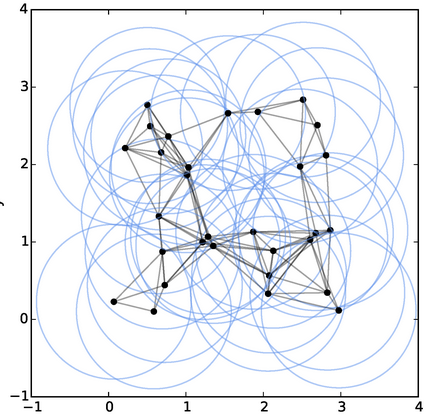
\includegraphics{WANET2.png}

\emph{Range of communication demonstrated by surrounding circle}

    \hypertarget{communication-scheme}{%
\section{Communication Scheme:}\label{communication-scheme}}

Each device uses radio waves to communicate packets to other devices.
The broadcasted message is transmitted between nodes over a certain
frequency channel. If two devices use the channel simulatenously, a
``collision'' occurs. This nullifies both broadcasts.

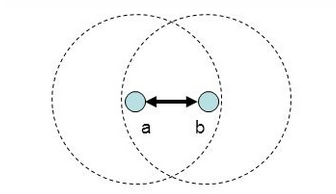
\includegraphics{interference.png}

\pagebreak

This can cause complex interactions amongst the communication nodes. For
example in the \emph{``hidden node problem''} (see below), node
\(N_{A}\) can see \(N_{B}\), but cannot see \(N_{C}\). If \(N_{A}\) and
\(N_{C}\) both communicate to \(N_{B}\) simultaneously, then a collision
will occur; furthermore, node \(N_{A}\) cannot attribute this collision
to \(N_{C}\) unless information is shared amongst the nodes.

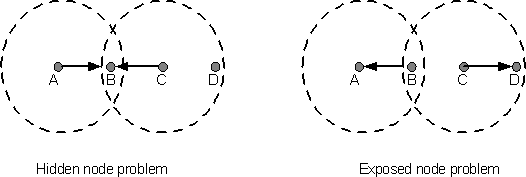
\includegraphics{hiddennode.png}

These interference problems coupled with a decentralized control scheme
can lead to inefficient routing. A large portion of time can be spent
rebroadcasting messages which previously collided.

    \hypertarget{traditional-solutions-abridged}{%
\section{Traditional Solutions
(abridged):}\label{traditional-solutions-abridged}}

\begin{enumerate}
\def\labelenumi{\arabic{enumi}.}
\item
  Reactive routing (AODV):

  \begin{itemize}
  \item
    This method is reactive because nodes do not save information
    regarding the entire network topology. They only maintain
    connections to local neighbors.
  \item
    Nodes periodically send ``hello'' messages to gain information about
    their immediate neighbors.
  \item
    Whenever a node wishes to send a packet through the network, it
    sends a ``route request'' (RREQ) to find a path to the destination.
    This request is passed along the network following a fixed protocol
    until the destination is found. Then the information is passed back
    through the network to the sending node. 
  \end{itemize}
\item
  Proactive routing (OLSR):

  \begin{itemize}
  \item
    This method is proactive as the nodes maintain a local ``image'' of
    the network's full topology.
  \item
    Nodes periodically send ``hello'' messages to gain information about
    their immediate neighbors.
  \item
    Additionally, nodes broadcast their local connections to the rest of
    the network through ``flooding''. Essentially, the information is
    spread to every connected node in the network by a fixed policy.
    ``Flooding'' can cause unnecessary transmission and cause packet
    collisions.
  \item
    With a local image of the network, a version of shortest path
    algorithm is applied to find a suitable path to the destination.
  \end{itemize}
\end{enumerate}

    \hypertarget{why-reinforcement-learning}{%
\pagebreak
\section{Why Reinforcement
Learning?:}\label{why-reinforcement-learning}}

\begin{itemize}
\tightlist
\item
  More direct, global combinatiorial optimization in a distributed
  fashion seems unlikely to scale effectively (finding the exact optimum
  is NP-hard I would imagine)
\item
  The ``best'' strategy given limited computation time and limited power
  usage is difficult to derive directly
\item
  RL agents can learn how to best encorporate available information at a
  node to improve routing (while maintaining constraints such as power
  usage)
\item
  RL agents can learn how to most effectively cooperate (direct analysis
  is difficult). Ex: how often and how much information should be shared
  amongst neighbors.
\item
  The computation time complexity of a DRL solution could potentially be
  smaller (i.e.~faster) than a more straightforward optimization
  algorithm (latency is important)
\end{itemize}

    \hypertarget{rl-problem-constraints}{%
\section{RL Problem Constraints:}\label{rl-problem-constraints}}

\begin{enumerate}
\def\labelenumi{\arabic{enumi}.}
\item
  Decentralized control
\item
  Multi-agent learning scheme
\item
  Full cooperation (protocol enforced)
\item
  Arbitrary intercommunication (with associated cost)
\end{enumerate}

    \hypertarget{physical-environmental-constraints}{%
\section{Physical / Environmental
Constraints}\label{physical-environmental-constraints}}

\begin{enumerate}
\def\labelenumi{\arabic{enumi}.}
\tightlist
\item
  Number of unique frequency channels \(N_{c}\) is variable and will be
  analyzed to see achievability of specific data rates
\item
  Range of unique frequency channels is proportional to transmission
  frequency
\end{enumerate}

    \hypertarget{rl-agent-state-space}{%
\section{RL Agent State Space:}\label{rl-agent-state-space}}

\begin{itemize}
\tightlist
\item
  there are a number of potential state types which may prove useful in
  deriving the best policy. Below is a list of state classes and
  specifics.
\end{itemize}

\begin{enumerate}
\def\labelenumi{\arabic{enumi}.}
\tightlist
\item
  Routing Information:

  \begin{itemize}
  \tightlist
  \item
    Packet source / destination
  \end{itemize}
\item
  Environment Information:

  \begin{itemize}
  \tightlist
  \item
    Current estimate of topology of network
  \item
    Strength of network connections
  \item
    Physical location and heading of nodes (possible?)
  \end{itemize}
\item
  System Information:

  \begin{itemize}
  \tightlist
  \item
    number packets in local buffer
  \item
    battery state
  \end{itemize}
\item
  History

  \begin{itemize}
  \tightlist
  \item
    time of day
  \item
    time elapsed between certain actions
  \end{itemize}
\end{enumerate}

    \hypertarget{rl-agent-action-space}{%
\section{RL Agent Action Space:}\label{rl-agent-action-space}}

\begin{itemize}
\tightlist
\item
  similar to the state space, there are a number of distinct actions
  which can be considered.
\item
  I would imagine that the action space should be structured as a
  sequence of decisions within time slots (viewed as a time series)
\end{itemize}

\begin{enumerate}
\def\labelenumi{\arabic{enumi}.}
\item
  Packet Related

  \begin{itemize}
  \tightlist
  \item
    Forward packet to neighbor (on specific channel)
  \item
    Drop packet
  \item
    Save packet to buffer
  \item
    WAIT (do nothing)
  \end{itemize}
\item
  Environment related

  \begin{itemize}
  \tightlist
  \item
    Sense channels (local connections)
  \item
    Measure local node locations (may not be physically feasable)
  \end{itemize}
\item
  Cooperation related

  \begin{itemize}
  \tightlist
  \item
    Proactively / reactively share information with nodes in network
  \item
    Proactively / reactively request information from network
  \end{itemize}
\end{enumerate}

    \hypertarget{reinforcement-signal-reinforcement-protocol}{%
\section{Reinforcement Signal / Reinforcement
Protocol}\label{reinforcement-signal-reinforcement-protocol}}

\begin{itemize}
\item
  the reinforcement signal should be related to the following:

  \begin{itemize}
  \tightlist
  \item
    Quality of service (QoS)
  \item
    Transmission slowdown / delay
  \item
    Power usage
  \item
    Transmission collisions
  \end{itemize}
\item
  How the reinforcement signal should be exactly formulated will require
  more considereation.
\item
  The way in which the reinforcement signal is provided to an agent is
  also an open question.
\end{itemize}

    \hypertarget{initial-rl-form}{%
\pagebreak
\section{Initial RL Formulation:}\label{initial-rl-form}}
Assume constraints from sections 6 and 7. The following is an initial attempt
at formulating the state space, action space, and learning mechanism. 

\subsection{State Space}
Let the state space be broken into two primary sections: 

\begin{enumerate}
\def\labelenumi{\arabic{enumi}.}
\item \underline{Environment state}

Let a node's estimate of the true environment state be represented by a directed graphical model $G(N,E)$ with nodes $N$ and edges $E$.

%%graphical model image

Each node $n \in N$ represents an agent within the assumed collaborative scheme. (Let $n_\ell$ represent the local agent).  Each edge $e \in E$ represents the communication channel connecting two nodes.

Each node $n \in \{N \diagup n_\ell\}$ will hold the following information:
\begin{itemize}
\item
node ID
\item
flag if node is a destination of packet in buffer
\item 
counter for time elapsed since last received topology information from node
\item
information regarding collisions between $n_\ell$ and $n \in \{N \diagup n_\ell\}$
\end{itemize}

\item \underline{Local buffer state}

\end{enumerate}

\subsection{Action Space}

\subsection{Learning Method}

    \hypertarget{random-thoughts}{%
\pagebreak
\section{References:}\label{references}}

    \hypertarget{random-thoughts}{%
\pagebreak
\section{Random Thoughts:}\label{random-thoughts}}

\begin{itemize}
\tightlist
\item
  nodes can ``sniff'' packets and infer the graph structure
\item
  nodes could proactively probe the network to learn its structure
  (causal graph inference)
\item
  sharing information with neighboring nodes comes at a cost

  \begin{itemize}
  \tightlist
  \item
    how can the agent's local information be shared at different sizes?
  \item
    essentially a variable-sized embedding?
  \end{itemize}
\item
  perhaps it is wise to share some information at times which are less
  busy? (offline learning)
\item
  it seems that the model complexity of each node in the network could
  be variable and dependent on its position in the network

  \begin{itemize}
  \tightlist
  \item
    less connected nodes probably are less important in the global
    optimization and thus require less information
  \item
    spend power most efficintly based on network position
  \end{itemize}
\item
  if a core model is shared amongst the agents, then it may improve
  coordination

  \begin{itemize}
  \tightlist
  \item
    each node can anticipate the actions of the others
  \item
    maybe some portion of the model is shared and another is not (role
    assignment)
  \end{itemize}
\item
  what about fairness?

  \begin{itemize}
  \tightlist
  \item
    for example, in a mobile phone network the users closest to the bay
    stations will receive higher traffic loads
  \item
    perhaps these methods make more sense in settings where fairness
    isn't as relevant (team strategy vs.~mutual cooperation)
  \end{itemize}
  
\item
  perhaps some information is always passed along as part of the packet header?
  Inspiration from ant colony optimization.
  
\end{itemize}

    % Add a bibliography block to the postdoc
    
    
    
    \end{document}
